% Standalone source for the hcinfer sandwich-efficiency computation diagram.
% The document class, font setup, arrow style, and the restrained
% blue/green/purple/grey palette are copied from scripts/tikz/workflow.tex.
% Compile with latexmk -pdf, then rasterize to PNG at 300 DPI with
% pdftools::pdf_convert(), exactly as scripts/04-diagrams.R already does.
\documentclass[border=5pt]{standalone}
\usepackage{amsmath}
\usepackage{tikz}
\usetikzlibrary{arrows.meta,backgrounds,calc,fit,positioning,shapes.geometric}

\definecolor{hcink}{HTML}{243746}
\definecolor{hcpage}{HTML}{FFFFFF}
\definecolor{hcapi}{HTML}{2C5F8A}
\definecolor{hcapifill}{HTML}{F2F6FA}
\definecolor{hccorecol}{HTML}{3D6B5D}
\definecolor{hccorefill}{HTML}{F3F7F5}
\definecolor{hcobject}{HTML}{6A5D84}
\definecolor{hcobjectfill}{HTML}{F6F4F8}
\definecolor{hcsupport}{HTML}{8A8F94}
\definecolor{hcsupportfill}{HTML}{F7F8FA}
\definecolor{hcline}{HTML}{6D7680}

\tikzset{
  hcstage/.style={
    draw=hcink,
    rounded corners=3pt,
    line width=0.55pt,
    fill=hcpage,
    align=center,
    inner xsep=6pt,
    inner ysep=5pt,
    font=\small,
    text=hcink
  },
  hcinput/.style={hcstage, draw=hcapi, fill=hcapifill, text width=22mm},
  hcupper/.style={hcstage, draw=hccorecol, fill=hccorefill, text width=33mm},
  hclower/.style={hcstage, draw=hcobject, fill=hcobjectfill, text width=38mm},
  hcsolve/.style={hcstage, draw=hcapi, fill=hcapifill, line width=0.8pt,
    text width=40mm},
  hcavoid/.style={
    draw=hcsupport,
    densely dashed,
    rounded corners=3pt,
    line width=0.5pt,
    fill=hcsupportfill,
    align=center,
    inner xsep=6pt,
    inner ysep=5pt,
    font=\scriptsize,
    text=hcink,
    text width=110mm
  },
  hcedge/.style={
    -{Stealth[length=2.2mm,width=1.6mm]},
    line width=0.55pt,
    color=hcline
  }
}

\begin{document}
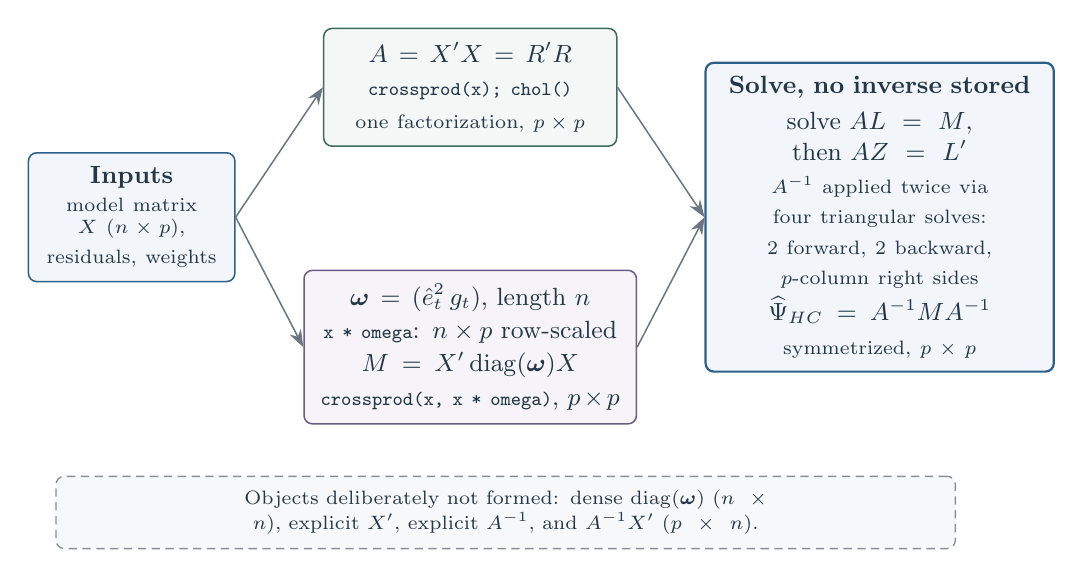
\begin{tikzpicture}[x=1cm,y=1cm]
  \node[hcinput] (in) at (0,0) {%
    \textbf{Inputs}\\[2pt]
    {\scriptsize model matrix $X$ ($n\times p$),\\ residuals, weights}%
  };

  \node[hcupper] (upper) at (4.3,1.65) {%
    $A=X'X=R'R$\\[1pt]
    {\scriptsize\ttfamily crossprod(x); chol()}\\[1pt]
    {\scriptsize one factorization, $p\times p$}%
  };

  \node[hclower] (lower) at (4.3,-1.65) {%
    $\boldsymbol{\omega}=(\hat e_t^2\, g_t)$, length $n$\\[1pt]
    {\scriptsize\ttfamily x * omega}: $n\times p$ row-scaled\\[1pt]
    $M=X'\operatorname{diag}(\boldsymbol{\omega})X$\\[1pt]
    {\scriptsize\ttfamily crossprod(x, x * omega)}, $p\times p$%
  };

  \node[hcsolve] (solve) at (9.5,0) {%
    \textbf{Solve, no inverse stored}\\[2pt]
    solve $AL=M$, then $AZ=L'$\\[1pt]
    {\scriptsize $A^{-1}$ applied twice via}\\
    {\scriptsize four triangular solves:}\\
    {\scriptsize 2 forward, 2 backward,}\\
    {\scriptsize $p$-column right sides}\\[2pt]
    $\widehat{\Psi}_{HC}=A^{-1}MA^{-1}$\\[1pt]
    {\scriptsize symmetrized, $p\times p$}%
  };

  \node[hcavoid] (avoid) at (4.75,-3.75) {%
    Objects deliberately not formed:
    dense $\operatorname{diag}(\boldsymbol{\omega})$ ($n\times n$),
    explicit $X'$, explicit $A^{-1}$, and $A^{-1}X'$ ($p\times n$).%
  };

  \draw[hcedge] (in.east) -- (upper.west);
  \draw[hcedge] (in.east) -- (lower.west);
  \draw[hcedge] (upper.east) -- (solve.west);
  \draw[hcedge] (lower.east) -- (solve.west);
\end{tikzpicture}
\end{document}
